%\vspace{-0.23in}
\chapter{Translator}
\label{sec:translator}
{\color{black}Given its popularity and ease of use \cite{Shankar2018,Godefroid2018,Thomsen2015,Groce2014}}, we build \sys using the Bandera Tool Set \cite{Hatcliff2001,Bandera:intro},
which is a collection of program analysis, transformation, and visualization components designed to apply
model-checking to verify Java source code.
Bandera generates a program model and specification in the language of one of several existing model-checking tools (including \spin, dSpin, SMV, JPF).
When a model-checker produces an error trail, Bandera renders the error trail at the source code level and allows the user to step through the code along the path of the trail while displaying values of variables and internal states of Java lock objects \cite{Hatcliff2001,Bandera:intro}.

Since Bandera %produces Promela code for \spin,
does not handle Groovy code, in order
to analyze smart apps for SmartThings, we need to convert their code into
Java which is challenging for the following reasons.
First, since SmartThings added several language features to Groovy to simplify smart app development,
the standard Groovy compiler cannot directly process an app's code
and SmartThings's compiler is not open sourced.
%Therefore, we need a module to convert from apps' code into standard Groovy code. Moreover, to translate the standard Groovy code.
Second, Groovy uses dynamic typing~\cite{Groovy:dynamic}
(\ie, data types are checked at run-time) but Java is static typed
(\ie, data types are explicitly declared and checked at compile-time).
Thus, we need to perform type inference during the translation of Groovy into Java.
Lastly, Groovy supports many built-in utilities such as list and map, not supported by Bandera
(\ie, Bandera supports only Java's \textit{array} type).

\begin{figure}[tb]
\begin{center}
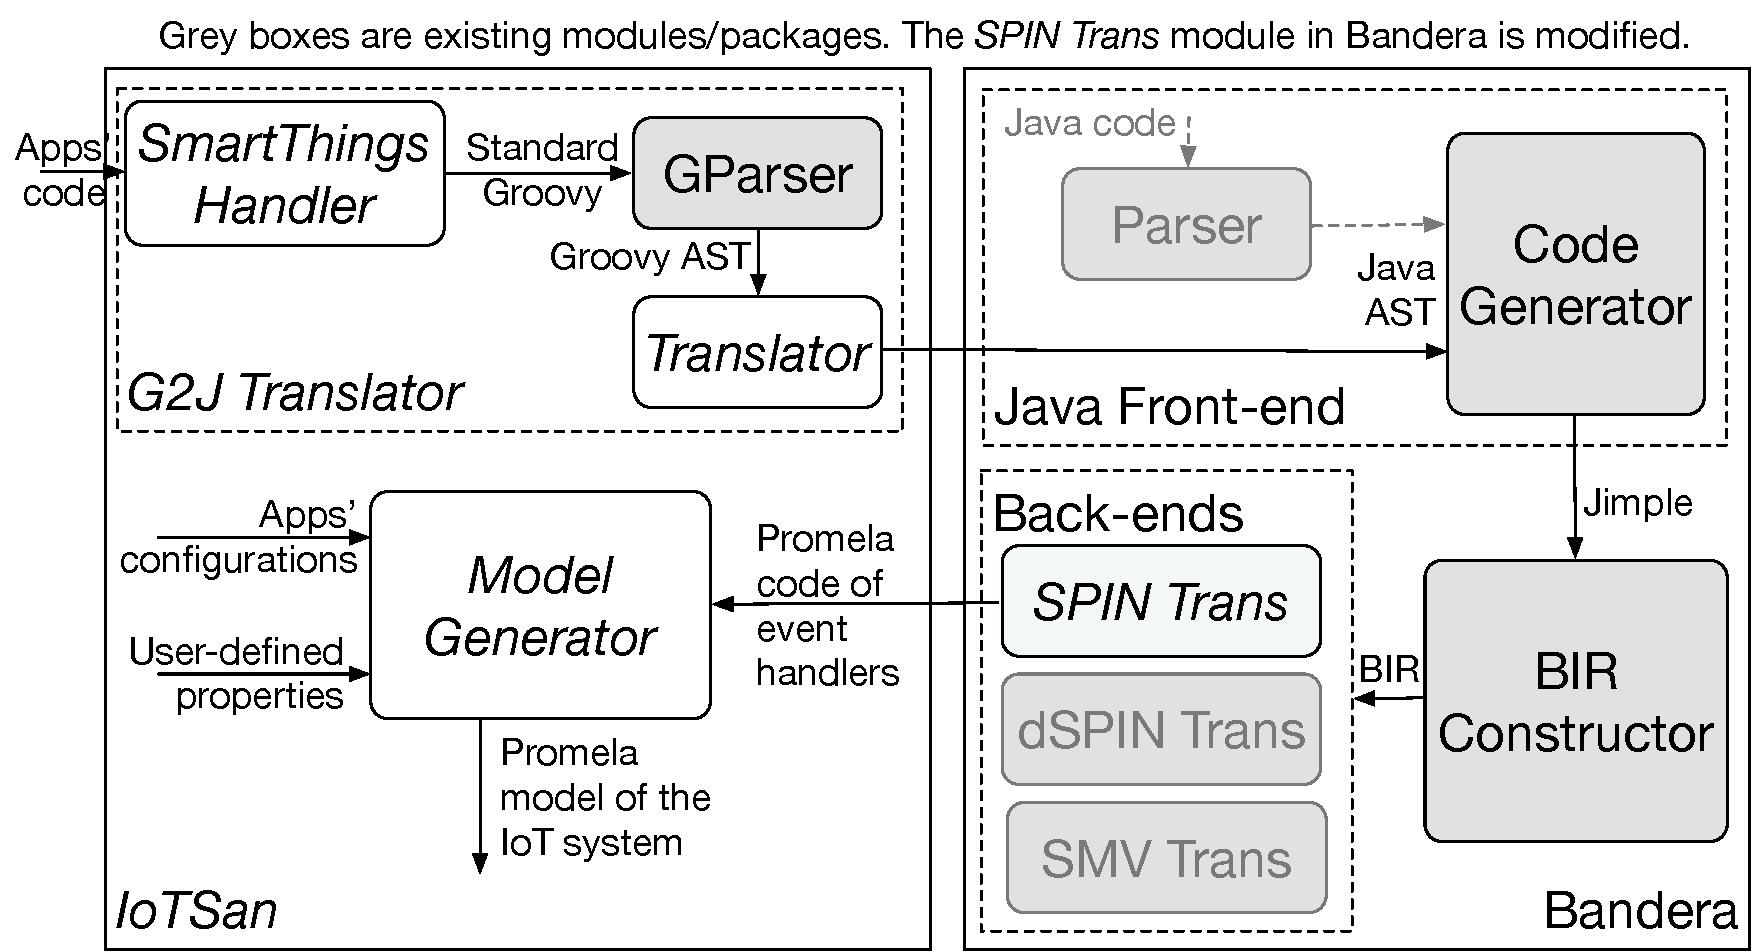
\includegraphics[width=3.8in]{IoTSanBanderaRelation}
%\vspace{-0.3in}
\caption{\textcolor{black}{\sys is built around Bandera.}}
%: the package \textit{org.codehaus.groovy} is used for the module GParser and the \textit{SPIN Trans} moduel in Bandera is modified.
\label{IoTSanBanderaRelation}
\end{center}
%\vspace{-0.25in}
\end{figure}


The key component we develop is the G2J Translator (see Figure~\ref{IoTSanBanderaRelation}),
which translates the smart app Groovy source into Java's Abstract Syntax Trees (ASTs).
In addition, the \textit{SmartThings Handler} is designed to handle the new language syntaxes introduced by SmartThings,
and the \textit{GParser} parses the regular Groovy source code into Groovy ASTs.
Basically, each smart app in Groovy is translated into a Java class,
whose method comprises of a method's header and a block of statements.
The translation procedure of a block is straightforward:
iterate through the statement list of the input Groovy block,
translate each Groovy statement into Java,
add the result to a list of Java statements,
and build a Java block from the result list.
To implement these,
we extended the Groovy compiler (\emph{org.codehaus.\allowbreak groovy})
which is then integrated into the Bandera's front-end.
%Below we describe how we address the above challenges.
%The translation procedure consists of two phases viz., (i) handling SmartThings' built-in utilities and (ii) translating Groovy's AST into Java's AST. Let us discuss this procedure in detail in the nutshell.

\section{Handling SmartThings' Language Features}
%Since SmartThings does not open the source code of its compiler, we build a library of SmartThings' platform based on their documentation \cite{Samsung:smartthingsapi}.
%Each object (\textit{e.g.}, attribute, command, capability, state, event, and device) is modeled by a Groovy class. All of these classes are packaged into a library, which is automatically imported by \textit{GParser} when parsing apps' source files.
There are several new language syntaxes introduced in SmartThings.
%examples of which are in Figure~\ref{inputexample}.
Our \textit{SmartThings Handler} parses these new syntaxes and converts them into
vanilla Groovy code using specifications based on the domain knowledge of SmartThings.
For instance, (as can be seen in {\color{black}in Figure~\ref{inputexample}) each $input$ function} defines a global variable (or a class field) of the app.
Therefore, we traverse the Groovy's AST of the app and visit all $input$ functions to extract all global variables of the app.
%$input$ method of SmartThings to get configuration information from users. Let us consider an example of an $input$ use case: \textit{input(name: ``color", type: ``enum", title: ``Color", options: [``Red",``Green",``Blue",``Yellow"])}, where $name$ defines the name of the variable that will be created in this smart app to reference this input; $type$ can be $capability.capabilityName$, $bool$, $decimal$, $email$, $enum$, $time$, $text$, $phone$, and so on; $option$ is a list of all possible values for this input.
In addition, apps can use some predefined objects or variables (\eg, $location$) and APIs (\eg, $setLocationMode$),
which are not defined in vanilla Groovy. Therefore, we manually add definitions of these global objects.
%Regarding their method definitions, we leave them as empty during the translation phase (so that the code compiles),
%but populate them during the modeling phase (see \S\ref{sec:model}).
%remove some SmartThings' built-in utilities (\textit{e.g.}, definition and preferences), which are not understandable by standard Groovy Compiler.

%\zhiyun{I'm not clear what we are doing here. After we extract the global variables from input, what do we do? Do we convert them into explicit variable definitions in Promela?}

%Moreover, an app can use some predefined variables, \textit{e.g.}, $location$, and APIs, \textit{e.g.}, $setLocationMode$. Then, we explicitly add definitions of the global variables as class fields and common APIs as local methods to the class of the app.

%: extract global variables used in the source file, and add definitions of these global variables and common SmartThings' objects (\textit{e.g.}, \textit{location} and APIs) to the source file;

%SmartThings allows apps to register callback functions (\textit{i.e.}, event handlers) - entry points of apps - for interested events via the $subscribe$ method. Since we need the info of event handlers in analyzing app dependency and generating Promela model, we also extract this info in this phase. Similar to the $input$ extraction, we also traverse the Groovy's AST of an app and visit all $subscribe$ method calls to get the subscribing info. \zhiyun{I understand that it is where you implement the callback function analysis, but this does not look like the translator's job. Can you check if this has anything to do with translation? The only thing I can image is that we may need to simulate the callback function ourselves because again the source code of the SmartThings framework is not available. However, logically I'd consider this more related to the modeling of the SmartThings system instead of part of the translator.}

\begin{figure}[tb]
	\ssp
    \centering
    %\raggedright
    \begin{subfigure}[t]{2.7in}
        \centering
        %\raggedleft
        %\includegraphics[width=1.3in]{groovycode}
		\lstinputlisting[language=groovy]{./code/groovycode.groovy}
		%\vspace{-0.12in}
        \caption{Groovy's code}
        \label{groovycode}
    \end{subfigure}\\
    %\vspace{-0.05in}
    \begin{subfigure}[t]{4.35in}
        \centering
        %\raggedleft
        %\includegraphics[width=2.4in]{javacode}
		\lstinputlisting[language=groovy]{./code/javacode.java}
				%\vspace{-0.12in}
        \caption{Corresponding Java's code}
        \label{javacode}
    \end{subfigure}
%\vspace{-0.1in}
    \caption{Example of translating a Groovy method into the corresponding Java's method.}
    \label{translationexample}
%\vspace{-0.22in}
\end{figure}

\section{Type Inference}
%{\color{red} We may use Gradual Typing with Unification-based Inference.}
%As mentioned above, Promela requires static typing of every declared variable, and therefore we need to perform type inference on Groovy code.
%\textit{org.codehaus.groovy}
Although the Groovy Compiler \textit{org.codehaus. groovy} already has a sub-package \textit{CompileStatic} for performing static type inference,
it only works when the argument type and the return type of a method are given.
In other words, a variable declared inside a method can take different runtime types depending on the argument type.
Thus, we still need to infer the argument and return type statically.
To do so, we consult the calling context of each method invocation
by recursively tracking the arguments and return values to their corresponding
anchor points---declaration of variables with explicit types (Groovy supports static typing as well),
assignment to constant values
(\eg, we can infer that the type of variable $a$ is numeric from \textit{def a = 0}),
assignment to return values of known APIs, and known objects and their properties.
The inference procedure works roughly as follows.
When traversing the AST of a method, we store the names and data types of variables at anchor points;
the types of other variables are inferred by propagating the types from anchor points.
This is done iteratively until we find no more new variables whose type can be inferred.


\section{Handling Groovy's Built-in Utilities}
%Another challenge is that since we are translating Groovy into Java which is then fed to Bandera.
Another challenge arises when we translate Groovy into Java for use with Bandera.
We find that Bandera understands only a very basic set of Java.
For instance, it supports only the $array$ type natively.
In contrast, Groovy's collection types (\eg, $Collection$, $List$, $ArrayList$, $Set$, $Map$, and $HashSet$)
all need to be translated into Java's $array$ type.
We support the popular collection types that are commonly used in smart apps.
An example is shown in Figure~\ref{translationexample} that translates one Groovy list into a corresponding Java implementation using array.
Since the type of \textit{switches} and \textit{onSwitches} is \textit{List of STSwtich},
we infer the return type of \textit{onSwitches()} method as \textit{List of STSwtich},
which is translated into Java's array type (\ie, \textit{STSwitch[]}).
The $+$ operation on \textit{List} type (line 2 in Figure~\ref{groovycode}) is
\textcolor{black}{automatically} translated into corresponding Java's code
(lines 2-17 in Figure~\ref{javacode}).
Finally, since this method is a non-void method,
we add an explicit $return$ statement (line 18 in Figure \ref{javacode}).





